\subsection{三角形全等的判定 III}\label{subsec:czjh1-3-7}

到现在为止,我们学过三种判定三角形全等的方法,即边角边公理,角边角公理以及推论角角边。
那么,是不是在两个三角形中,有任意三组对应的边或角相等时,两个三角形就全等呢?看下面几种情况。

例如,在 $\triangle ABC$ 和 $\triangle ABD$ 中,已知 $AB = AB$, $AC = AD$,
$\angle B = \angle B$,显然它们不全等(图 \ref{fig:czjh1-3-25})。 这说明,
两边和其中一边的对角对应相等的两个三角形不一定全等。

\begin{figure}[htbp]
    \centering
    \begin{minipage}[b]{7cm}
        \centering
        \begin{tikzpicture}
    \tkzDefPoints{0/0/B, 3.5/0/D, 2.8/2.5/A}
    \tkzInterLC(B,D)(A,D)  \tkzGetFirstPoint{C}

    \tkzDrawPolygon(A,B,D)
    \tkzDrawSegments(A,C)
    \tkzMarkSegments[mark=|](A,C  A,D)
    \tkzLabelPoints[above](A)
    \tkzLabelPoints[below](B,C,D)
\end{tikzpicture}


        \caption{}\label{fig:czjh1-3-25}
    \end{minipage}
    \qquad
    \begin{minipage}[b]{7cm}
        \centering
        \begin{tikzpicture}
    \tkzDefPoints{0/0/B, 3.5/0/C, 2.8/2.5/A}
    \tkzDefPointOnLine[pos=0.7](A,B)  \tkzGetPoint{D}
    \tkzDefPointOnLine[pos=0.7](A,C)  \tkzGetPoint{E}

    \tkzDrawPolygon(A,B,C)
    \tkzDrawSegments(D,E)
    \tkzLabelPoints[above](A)
    \tkzLabelPoints[left](B,D)
    \tkzLabelPoints[right](C,E)
\end{tikzpicture}


        \caption{}\label{fig:czjh1-3-26}
    \end{minipage}
\end{figure}

又如, 在 $\triangle ABC$ 和 $\triangle ADE$ 中,如果 $DE \pingxing BC$,
那么 $\angle ADE = \angle B$, $\angle AED = \angle C$, 又 $\angle A = \angle A$,
但 $\triangle ABC$ 和 $\triangle ADE$ 并不全等(图 \ref{fig:czjh1-3-26})。
这说明三个角对应相等的两个三角形也不一定全等。

但是,如果两个三角形的三条边对应相等,这两个三角形一定全等。
这个事实以后可以证明,所以有下面的定理:

\begin{dingli}[边边边定理]
    有三边对应相等的两个三角形全等
\end{dingli}(可以简写成 “\zhongdian{边边边}” 或 “$\bm{SSS}$”)。

例如,在图 \ref{fig:czjh1-3-27} 的 $\triangle ABC$ 和 $\triangle A'B'C'$ 中,如果
$BC = B'C'$, $CA = C'A'$, $AB = A'B'$, 那么
$$ \triangle ABC \quandeng \triangle A'B'C' \juhao $$

\begin{figure}[htbp]
    \centering
    \begin{minipage}[b]{9cm}
        \centering
        \begin{tikzpicture}
    % 两个 scope 的区别,仅仅在于各点的名称不同。
    % 所以将绘制代码抽取出来(复用)
    \def\drawtriangle{
        \tkzDefPoints{0/0/B, 3.5/0/C, 2.8/2/A}
        \tkzDrawPolygon(A,B,C)
        \tkzMarkSegment[mark=|](A,B)
        \tkzMarkSegment[mark=||](B,C)
        \tkzMarkSegment[mark=|||](A,C)
    }

    \begin{scope}
        \drawtriangle
        \tkzLabelPoints[above](A)
        \tkzLabelPoints[below](B,C)
    \end{scope}

    \begin{scope}[xshift=4.5cm]
        \drawtriangle
        \tkzLabelPoint[above](A){$A'$}
        \tkzLabelPoint[below](B){$B'$}
        \tkzLabelPoint[below](C){$C'$}
    \end{scope}
\end{tikzpicture}


        \caption{}\label{fig:czjh1-3-27}
    \end{minipage}
    \qquad
    \begin{minipage}[b]{5cm}
        \centering
        \begin{tikzpicture}
    \tkzDefPoints{0/0/A,  3/0/B,  0.5/2/D, 3.5/2/C}
    \tkzDefPointOnLine[pos=0.3](A,C)  \tkzGetPoint{E}
    \tkzDefPointOnLine[pos=0.3](C,A)  \tkzGetPoint{F}

    \tkzDrawPolygon(A,B,C,D)
    \tkzDrawSegments(A,C  D,E  B,F)
    \tkzMarkAngles[size=0.5](A,C,B  C,A,D)
    \tkzLabelAngle[pos=0.8](A,C,B){$1$}
    \tkzLabelAngle[pos=0.8](C,A,D){$2$}
    \tkzLabelPoints[left](A,D)
    \tkzLabelPoints[right](B,C)
    \tkzLabelPoints[below, xshift=0.3em](E)
    \tkzLabelPoints[above, xshift=-0.3em](F)
\end{tikzpicture}


        \caption{}\label{fig:czjh1-3-28}
    \end{minipage}
\end{figure}


\liti[0] 已知:如图 \ref{fig:czjh1-3-28},$AB = CD$, $BC = DA$, $E$、 $F$ 是 $AC$ 上两点,且 $AE = CF$。

求证: $BF = DE$。

\zhengming 在 $\triangle ABC$ 和 $\triangle CDA$ 中,

\hspace{2em}$\begin{cases}
    AB = CD & \text{(已知),} \\
    BC = DA & \text{(已知),} \\
    CA = AC & \text{(公共边),} \\
\end{cases}$

$\therefore$ \quad $\triangle ABC \quandeng \triangle CDA$ ($SSS$) 。

$\therefore$ \quad $\angle 1 = \angle 2$ (全等三角形的对应角相等)。

在 $\triangle BCF$ 和 $\triangle DAE$ 中,

\hspace{2em}$\begin{cases}
    BC = DA  & \text{(已知),} \\
    \angle 1 = \angle 2 & \text{(已证),} \\
    CF = AE & \text{(已知),} \\
\end{cases}$

$\therefore$ \quad $\triangle BCF \quandeng \triangle DAE$ ($SAS$) 。

$\therefore$ \quad $BF = DE$ (全等三角形的对应边相等)。


由边边边定理可以看出,只要三角形三边的长度固定,这个三角形的形状大小就完全确定。
例如,取三根长度适当的木条,用钉子把它们钉成一个三角形框架,
所得到的框架形状和大小就固定了( 图 \ref{fig:czjh1-3-29})。
三角形这个性质叫做\zhongdian{三角形的稳定性}。这是三角形特有的性质。
用四根木条钉成的框架就没有这个性质,它的形状是可以改变的(图 \ref{fig:czjh1-3-30})。

\begin{figure}[htbp]
    \centering
    \begin{minipage}[b]{7cm}
        \centering
        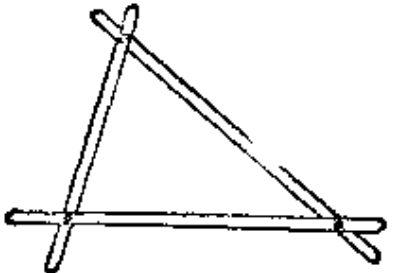
\includegraphics[width=5cm]{../pic/czjh1-ch3-29.png}
        \caption{}\label{fig:czjh1-3-29}
    \end{minipage}
    \qquad
    \begin{minipage}[b]{7cm}
        \centering
        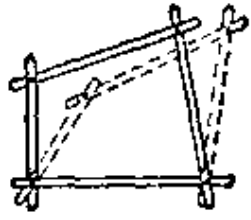
\includegraphics[width=4cm]{../pic/czjh1-ch3-30.png}
        \caption{}\label{fig:czjh1-3-30}
    \end{minipage}
\end{figure}


三角形的稳定性在生产和生活中是很有用的。
例如,房屋的人字梁具有三角形的结构,它就坚固和稳定;
在栅栏门上斜着钉一条(或两条)木板,构成一些三角形,就可以使栅栏门不变形。
前面提到的大桥钢梁、起重机的支架都采用三角形结构,也是这个道理。


\begin{lianxi}

\xiaoti{如图是一个平分角的仪嚣,其中 $AB = AD$, $BC = DC$。
    为了平分一个角,只要将点 $A$ 放在角的顶点, $AB$ 和 $AD$ 沿角的两边放下,
    沿 $AC$ 画一射线 $AE$, $AE$ 就是角平分线。说明它的道理。
}

\begin{figure}[htbp]
    \centering
    \begin{minipage}[b]{4cm}
        \centering
        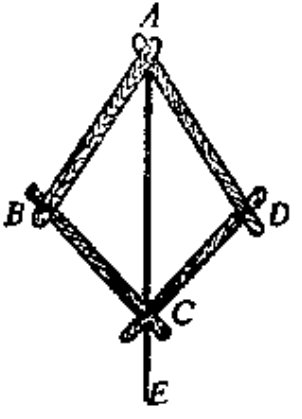
\includegraphics[width=3cm]{../pic/czjh1-ch3-subsec7-lx-01.png}
        \caption*{(第 1 题)}
    \end{minipage}
    \qquad
    \begin{minipage}[b]{4.5cm}
        \centering
        \begin{tikzpicture}
    \tkzDefPoints{0/0/B,  2.5/0/C,  1/0/E, 3.5/0/F, 0.8/2/A,  1.8/2/D}

    \tkzDrawPolygon(A,B,C)
    \tkzDrawPolygon(D,E,F)
    \tkzLabelPoints[above](A,D)
    \tkzLabelPoints[below](B,E,C,F)
\end{tikzpicture}


        \caption*{(第 2 题)}
    \end{minipage}
    \qquad
    \begin{minipage}[b]{4.5cm}
        \centering
        \begin{tikzpicture}[scale=0.9]
    \tkzDefPoints{0/0/B,  3/0/C,  0.8/2/A, 3.8/2/D}

    \tkzDrawPolygon(A,B,C,D)
    \tkzLabelPoints[left](B)
    \tkzLabelPoints[right](C)
    \tkzLabelPoints[above](A,D)
\end{tikzpicture}


        \caption*{(第 3 题)}
    \end{minipage}
\end{figure}


\xiaoti{已知:如图,点 $B$、$E$、$C$、$F$ 在同一直线上,$AB = DE$, $AC = DF$, $BE = CF$。 \\
    求证: $\angle A = \angle D$。
}

\xiaoti{已知:如图, $AB = DC$, $AD = BC$。 \\
    求证: $\angle A = \angle C$。
}

\xiaoti{举出一些利用三角形稳定性的实例。}

\end{lianxi}

